\documentclass[11pt,fleqn]{article}
\usepackage[margin=1in,top=1in,bottom=1in]{geometry}
\usepackage{tikz}
\usepackage{mathtools}
\usepackage{longtable}
\usepackage{enumitem}
\usepackage{hyperref}
%\usepackage[dvips]{graphics}
%\usepackage[table]{xcolor}
%\usepackage{amssymb}
\usepackage{float}
%\usepackage{subfig}
\usepackage{booktabs}
\usepackage{subcaption}

\usepackage[normalem]{ulem}

\usepackage{multicol}
\usepackage{txfonts}
\usepackage{amsfonts}
\usepackage{natbib}
\usepackage{gb4e}
\usepackage[all]{xy}
\usepackage{rotating}
\usepackage{tipa}
\usepackage{multirow}
\usepackage{authblk}
\usepackage{url}
\usepackage{pdflscape}
\usepackage{rotating}
\usepackage{adjustbox}
\usepackage{array}


\def\bad{{\leavevmode\llap{*}}}
\def\marginal{{\leavevmode\llap{?}}}
\def\verymarginal{{\leavevmode\llap{??}}}
\def\swmarginal{{\leavevmode\llap{4}}}
\def\infelic{{\leavevmode\llap{\#}}}

\definecolor{airforceblue}{rgb}{0.36, 0.54, 0.66}
%\definecolor{gray}{rgb}{0.36, 0.54, 0.66}

\definecolor{Pink}{RGB}{240,0,120}
\newcommand{\red}[1]{\textcolor{Pink}{#1}}
\newcommand{\jd}[1]{\textbf{\textcolor{Pink}{[jd: #1]}}}

\newcommand{\dashrule}[1][black]{%
  \color{#1}\rule[\dimexpr.5ex-.2pt]{4pt}{.4pt}\xleaders\hbox{\rule{4pt}{0pt}\rule[\dimexpr.5ex-.2pt]{4pt}{.4pt}}\hfill\kern0pt%
}

\setlength{\parindent}{.3in}
\setlength{\parskip}{0ex}

\newcommand{\yi}{\'{\symbol{16}}}
\newcommand{\nasi}{\~{\symbol{16}}}
\newcommand{\hina}{h\nasi na}
\newcommand{\ina}{\nasi na}

\newcommand{\foc}{$_{\mbox{\small F}}$}

\hyphenation{par-ti-ci-pa-tion}

\setlength{\bibhang}{0.5in}
\setlength{\bibsep}{0mm}
\bibpunct[:]{(}{)}{,}{a}{}{,}

\newcommand{\6}{\mbox{$[\hspace*{-.6mm}[$}} 
\newcommand{\9}{\mbox{$]\hspace*{-.6mm}]$}}
\newcommand{\sem}[2]{\6#1\9$^{#2}$}
\renewcommand{\ni}{\~{\i}}

\newcommand{\citepos}[1]{\citeauthor{#1}'s \citeyear{#1}}
\newcommand{\citeposs}[1]{\citeauthor{#1}'s}
\newcommand{\citetpos}[1]{\citeauthor{#1}'s (\citeyear{#1})}

\newcolumntype{R}[2]{%
    >{\adjustbox{angle=#1,lap=\width-(#2)}\bgroup}%
    l%
    <{\egroup}%
}
\newcommand*\rot{\multicolumn{1}{R{90}{0em}}}% no optional argument here, please!


\title{Does at-issueness predict projection? Further investigations of the Gradient Projection Principle}

%\thanks{For helpful comments on the research presented here, we thank David Beaver, Cleo Condoravdi, Kai von Fintel, Lauri Karttunen, Mandy Simons, Greg Scontras, the anonymous reviewers for {\em Semantics and Linguistic Theory} 2018, as well as the audiences at the MIT Linguistics colloquium, the 2018 Annual Meeting of XPRAG.de and at the University of T\"ubingen. We gratefully acknowledge financial support for this research from {\em National Science Foundation} grant BCS-1452674 (JT) and the Targeted Investment for Excellence Initiative at The Ohio State University (JT). IGOR Tuebingen, SALT TALK}}

\author{Author(s)}

%\author[$\circ$]{Judith Tonhauser}
%\author[$\bullet$]{Judith Degen}
%\affil[$\circ$]{The Ohio State University / University of Stuttgart}
%\affil[$\bullet$]{Stanford University}
%
%\renewcommand\Authands{ and }

\newcommand{\jt}[1]{\textbf{\color{blue}JT: #1}}

\begin{document}

%\tableofcontents
%\newpage

\maketitle

\vspace*{-1cm}

\begin{abstract}

\citealt{tbd-variability} hypothesized that at-issueness is one factor that modulates the projection of content (see also \citealt{brst-salt10,brst-ar}). Specifically, according to their Gradient Projection Principle, if content $C$ is expressed by a constituent embedded under an entailment-canceling operator, then $C$ projects to the extent that it is not at-issue. Their work provided evidence for the GPP from xx contents that had been described as projective in the literature, at-issueness was measured in two different ways, only one consistently brought evidence in support (question, asking whether, are you sure? mixed results 2b). This paper provides further investigate the GPP by investigating a) more varied items, b) with more types of embedding, and c) other measures of at-issueness. These experiments provide additional support for the GPP, and they also show: comparison of projection across entailment-canceling operators, comparison of at-issueness diagnostics. Suggests that the diagnostics may not all measure the same (\citealt{snider2017}).

\end{abstract}

		
\section{Introduction}\label{s1}

\begin{exe}
\ex\label{gpp} {\bf Gradient Projection Principle} \hfill (\citealt[400]{tbd-variability}) \\ If content $C$ is expressed by a constituent embedded under an entailment-canceling operator, then $C$ projects to the extent that it is not at-issue.
\end{exe}


\begin{exe}
\ex\label{rqs} {\bf Main research question} \\
Are not-at-issueness and projection positively correlated, as predicted by the Gradient Projection Principle?
\end{exe}

\begin{exe}
\ex\label{rqs} {\bf Ancillary research questions}
\begin{xlist}
\ex Is the projection of contents embedded under different entailment-canceling operators positively correlated, as assumed in the semantics/pragmatics literature?

\ex Is the at-issueness of contents embedded under different entailment-canceling operators positively correlated?

\ex Is the at-issueness of contents positively correlated under different measures of at-issueness?
\end{xlist}
\end{exe}

\section{Prior literature}\label{s2}

\begin{exe}
\ex\label{pred} 20 clause-embedding predicates 

\begin{xlist}

\ex canonically factive: {\em be annoyed, discover, know, reveal, see}

\ex nonfactive:

\begin{xlist}

\ex nonveridical nonfactive: {\em pretend, suggest, say, think}

\ex veridical nonfactive: {\em be right, demonstrate}

\end{xlist}

\ex optionally factive: {\em acknowledge, admit, announce, confess, confirm, establish, hear, inform, prove}

\end{xlist}

\end{exe}

\section{Experiments 1-3: Methods}\label{s3}

Exps.~1a and 1b were designed to investigate which of the CCs of the 20 clause-embedding predicates in \ref{pred} are presupposed.\footnote{\label{f-github}The experiments, data, and R code for generating the figures and analyses of the experiments reported in this paper are available at \url{https://github.com/judith-tonhauser/projective-probability}. All experiments were conducted with IRB approval. Exps.~1b, 2b, and 3b were preregistered: \url{https://osf.io/cxq47}.}

The experiments employed the {\sc certain that} diagnostic for projection (see also, e.g.\ \citealt{tonhauser-salt26,djaerv-bacovcin-salt27,stevens-etal2017,lorson2018,tbd-variability,mahler-nels,mahler2020,demarneffe-etal-sub23}): on this diagnostic, participants are presented with an utterance in which the content to be investigated occurs in an entailment-canceling environment, like a polar question, as illustrated in \ref{stim} for the content of the appositive, that Martha's new car is a BMW.\footnote{For other diagnostics for projection see, e.g.\ \citealt{smith-hall11,xue-onea11}, and \citealt{brst-lang11}; see also the discussion in \citealt{tbd-variability}.} 

\begin{exe}

\ex\label{stim} Patrick asks: {\em Was Martha's new car, a BMW, expensive?} 

\end{exe}
To assess projection, participants are asked whether the speaker is certain of the content; for instance, in \ref{stim}, participants are asked whether Patrick is certain that Martha's new car is a BMW. If a participant takes the speaker to be certain of the content, we assume that the content projects, that is, the content is presupposed by the speaker; if a participant does not take the speaker to be certain of the content, we assume that the content does not project, that is, the content is not presupposed.

Following \citealt{tbd-variability}, Exp.~1a implemented the certain that diagnostic with a gradient response scale: participants gave their responses on a slider marked `no' at one end and `yes' at the other. We assume that the closer to `yes' a participant's response is, the more the speaker is certain of the content, that is, the more projective the content is. In other words, we assume that gradient certainty ratings reflect gradience in the speaker's commitment to the truth of the content.\footnote{Strictly speaking,  gradient certainty ratings reflect gradience in the degree to which participants \emph{perceive} the speaker to be committed to the truth of the content. That is, as in any experiment, the quantity of interest, in this case speaker commitment, is only indirectly measured.} As discussed in \citealt{tbd-variability}, a second interpretation of gradient certainty ratings is that they reflect a participant's degree of belief in the speaker's (binary) commitment to the truth of the content. While we adopt the first interpretation in our discussion, we remain agnostic about the interpretation of gradient certainty ratings: either interpretation gives rise to the expectation,  on the definition of factive predicates in \ref{def}a, that certainty ratings for factive predicates are categorically higher than for optionally factive and nonfactive ones. 

Exp.~1b was identical to Exp.~1a but employed a two-alternative forced choice task where participants categorically responded `yes' or `no'.

\subsection{Participants}

We recruited 250-300 participants for each of Exps.~1-3. Participants for Exp.~1q were recruited on Amazon's Mechanical Turk platform; the participants were required to have U.S.\ IP addresses and at least 99\% of previously approved HITs. Participants for the remaining experiments were recruited on Prolific; these participants were required to reside in the US, to be born in the US, to have English as their first language, and to have an approval rating of at least 99\%. Information on recruited participants (total number, ages, gender) and the payments they received can be found in Supplement \ref{a-participants}.

\subsection{Materials}

Exps.~1-3 investigated the projection and at-issueness of the CC of the 20 clause-embedding predicates in (\ref{pred}). The clausal complements of the 20 predicates were realized by 20 clauses (provided in Supplement \ref{a-clauses}), for a total of 400 predicate/clause combinations. These 400 predicate/clause combinations were combined with proper name subjects (a unique name per complement clause) to realize polar questions (in Exps. 1q, 2q, and 3q), negated declaratives (in Exps. 1n, 2n, and 3n), declaratives with the modal adverb {\em perhaps} (in Exps. 1m, 2m, and 3m), and the antecedents of conditionals (in Exps. 1c, 2c, and 3c). These sentences were presented as utterances by a named speaker. A sample set of target utterances is given in (\ref{sample-stims}): here, the named speaker is {\em Daniel}, the subject of the clause-embedding predicate is {\em Cole}, the predicate is {\em discover}, and the complement clause is {\em Julian dances salsa}.\footnote{The indirect object of {\em inform} was realized by the proper name {\em Sam}. The predicates differed in the tense in which they were realized. In polar interrogatives as well as in negated and modalized declaratives, eventive predicates, like {\em discover} and {\em hear}, were realized in the past tense and stative predicates, like {\em know} and {\em be annoyed}, were realized in the present tense.  In the antecedents of conditionals, all predicates were realized in the present tense. For the consequents of the conditional sentences see Supplement \ref{a-target}.}

\begin{exe}
\ex\label{sample-stims}
\begin{xlist}
\ex {\bf Daniel:} ``{\em Did Cole discover that Julian dances salsa?}"
\ex {\bf Daniel:} ``{\em Cole didn't discover that Julian dances salsa.}"
\ex {\bf Daniel:} ``{\em Perhaps Cole discovered that Julian dances salsa.}"
\ex {\bf Daniel:} ``{\em If Cole discovered that Julian dances salsa, Logan will be joyful.}"
\end{xlist}
\end{exe}
The proper names that realized the speakers, the subjects of the clause-embedding predicates, the subjects of the complement clauses, and the subjects of the consequents  were all unique.

Projection and at-issueness of the contents of the clausal complements were measured in separate blocks. In the projection blocks across Exps.~1-3, projection was measured with the `certain that' diagnostic. The target stimuli consisted of the target utterances, as shown in Figure \ref{f-projection-trials}.


\begin{figure}[h!]
\centering

\begin{subfigure}[t]{0.5\textwidth}
        \centering
\fbox{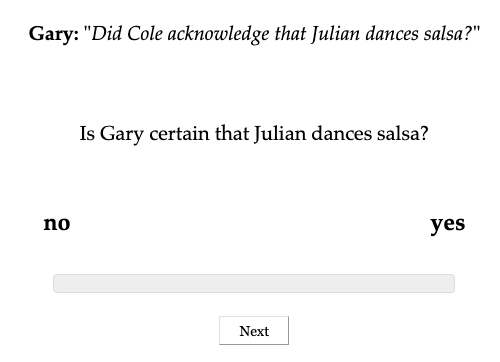
\includegraphics[height=4.4cm,width=7.6cm]{figures/2q-proj}}
\caption{Exps.~1q, 2q, and 3q.}\label{fig-exp1q-projection}
\end{subfigure}%
\begin{subfigure}[t]{0.5\textwidth}
\centering
\fbox{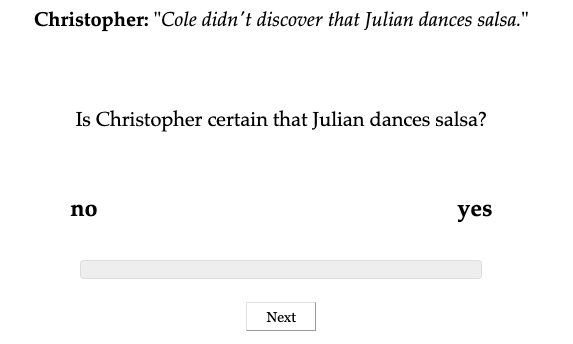
\includegraphics[height=4.4cm,width=7.6cm]{figures/1n-proj}} 
\caption{Exps.~1n, 2n, and 3n.}\label{fig-exp1n-projection}
 \end{subfigure}
\begin{subfigure}[t]{0.5\textwidth}
        \centering
\fbox{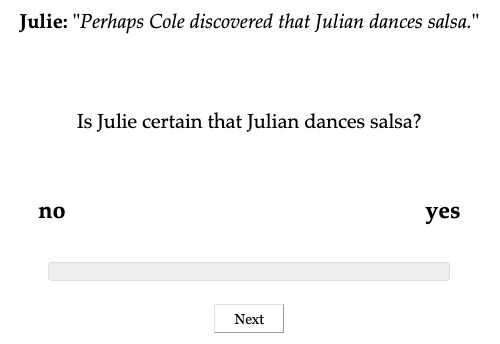
\includegraphics[height=4.4cm,width=7.6cm]{figures/1m-proj}}
\caption{Exps.~1m, 2m, and 3m}\label{fig-exp1m-projection}
 \end{subfigure}%
\begin{subfigure}[t]{0.5\textwidth}
\centering
\fbox{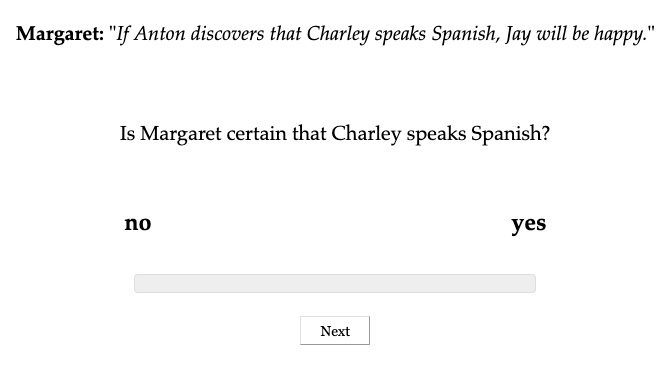
\includegraphics[height=4.4cm,width=7.6cm]{figures/1c-proj}} 
\caption{Exps.~1c, 2c, and 3c}\label{fig-exp1c-projection}
\end{subfigure}


\caption{Target trials in projection blocks of Exps.~1, 2, and 3 for the complement {\em Julian dances salsa}.}\label{f-projection-trials}
\end{figure}

The at-issueness diagnostics differed between Exps.~1, 2, and 3: at-issueness was measured in Exp.~1q, 2q, and 3q, with variants of the question-based diagnostic of at-issueness, namely the `asking whether' diagnostic in Exp.~1q, and the `yes, $p$' diagnostic in Exps.~2q and 3q, as shown in Figure \ref{fig-ai-trials-q}.


, with the `sure that' diagnostic in Exps.~1n, 1m, and 1c, with the `yes' diagnostic in Exps.~2q and 3q, with the `assent with positive continuation' diagnostic in Exps.~2n, 2m, and 2c,  and with the `assent with adversative continuation' diagnostic in Exps.~3n, 3m, and 3c.  


To assess whether participants were attending to the task, each experiment also included six control stimuli, which were also utterances made by a named speaker. (The controls are provided in Supplement \ref{a-control}.) Each participant saw a random set of 26 stimuli: each set contained one target utterance for each of the 20 clause-embedding predicates (each with a unique complement clause) and the same 6 control stimuli. Each participant saw their set of 26 stimuli twice, once in the projection block and once in the at-issueness block. Block order and within-block trial order was randomized. 


\begin{figure}[h!]
\centering

\begin{subfigure}[t]{0.5\textwidth}
        \centering
\fbox{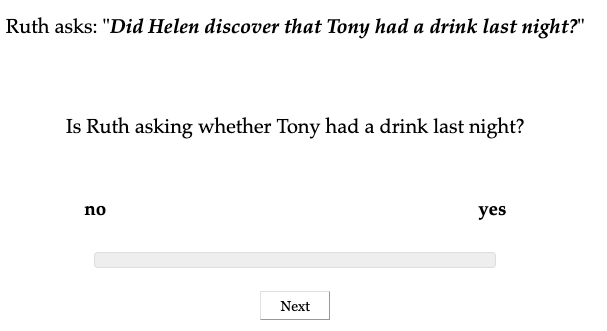
\includegraphics[height=5.4cm,width=7.6cm]{figures/1q-ai}}
\caption{Exp.~1q.}\label{fig-exp1q-ai}
\end{subfigure}
\begin{subfigure}[t]{0.5\textwidth}
\centering
\fbox{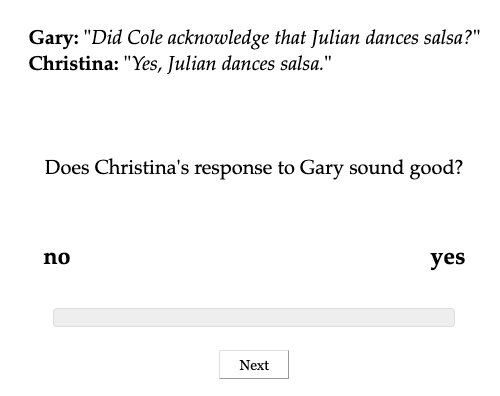
\includegraphics[height=5.4cm,width=7.6cm]{figures/2q-ai}} 
\caption{Exp.~2q.}\label{fig-exp2q-ai}
 \end{subfigure}%
\begin{subfigure}[t]{0.5\textwidth}
        \centering
\fbox{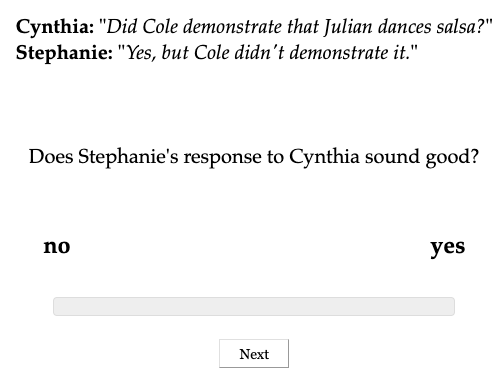
\includegraphics[height=5.4cm,width=7.6cm]{figures/3q-ai}}
\caption{Exp.~3q}\label{fig-exp3q-ai}
 \end{subfigure}

\caption{Target trials in at-issueness blocks of Exps.~1q, 2q, and 3q for the complement {\em Julian dances salsa}.}\label{f-ai-trialsq}
\end{figure}

\begin{figure}[h!]
\centering

\begin{subfigure}[t]{0.5\textwidth}
        \centering
\fbox{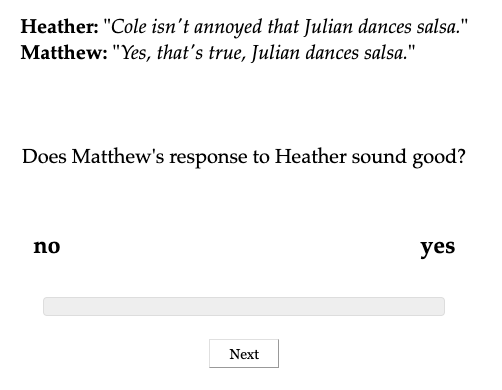
\includegraphics[height=5.4cm,width=7.6cm]{figures/2n-ai}}
\caption{Exp.~2n.}\label{fig-exp1q-ai}
\end{subfigure}%
\begin{subfigure}[t]{0.5\textwidth}
\centering
\fbox{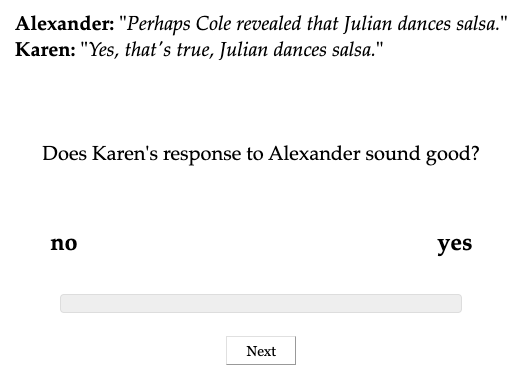
\includegraphics[height=5.4cm,width=7.6cm]{figures/2m-ai}} 
\caption{Exp.~2m.}\label{fig-exp2q-ai}
 \end{subfigure}
\begin{subfigure}[t]{0.5\textwidth}
        \centering
\fbox{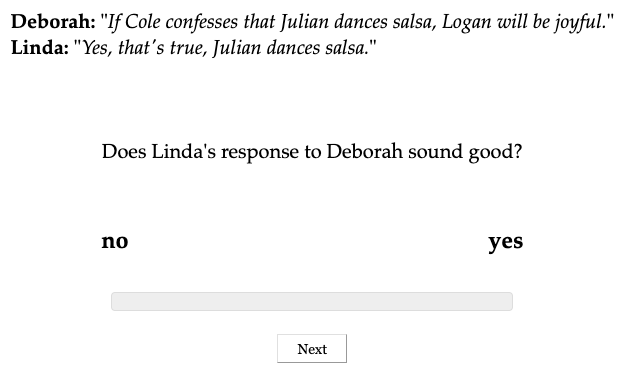
\includegraphics[height=5.4cm,width=9cm]{figures/2c-ai}}
\caption{Exp.~2c}\label{fig-exp3q-ai}
 \end{subfigure}

\caption{Target trials in at-issueness blocks of Exps.~2n, 2m, and 2c for the complement {\em Julian dances salsa}.}\label{f-ai-trialsq}
\end{figure}


\begin{figure}[h!]
\centering

\begin{subfigure}[t]{0.5\textwidth}
        \centering
\fbox{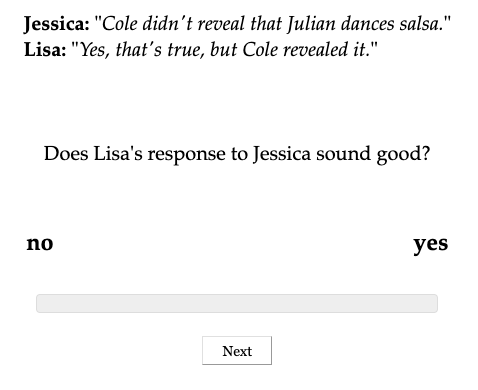
\includegraphics[height=5.4cm,width=7.6cm]{figures/3n-ai}}
\caption{Exp.~3n.}\label{fig-exp1q-ai}
\end{subfigure}%
\begin{subfigure}[t]{0.5\textwidth}
\centering
\fbox{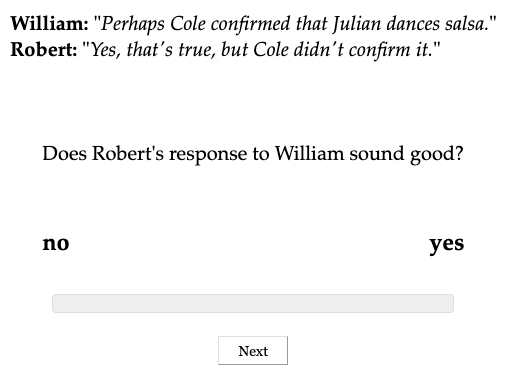
\includegraphics[height=5.4cm,width=7.6cm]{figures/3m-ai}} 
\caption{Exp.~3m.}\label{fig-exp2q-ai}
 \end{subfigure}
\begin{subfigure}[t]{0.5\textwidth}
        \centering
\fbox{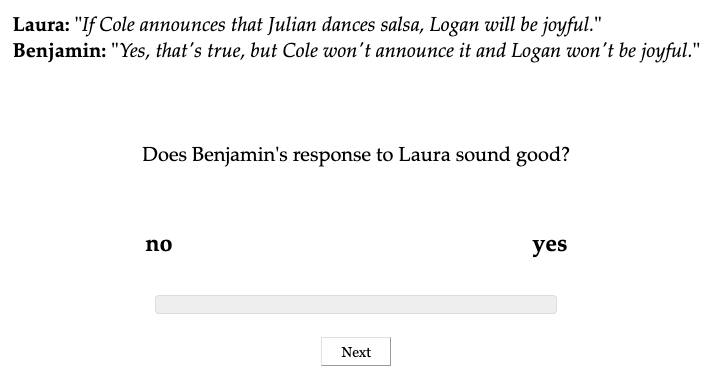
\includegraphics[height=5.4cm,width=9cm]{figures/3c-ai}}
\caption{Exp.~3c}\label{fig-exp3q-ai}
 \end{subfigure}

\caption{Target trials in at-issueness blocks of Exps.~3n, 3m, and 3c for the complement {\em Julian dances salsa}.}\label{f-ai-trialsq}
\end{figure}


In the projection block, target stimuli consisted of a fact and a polar question that was ut- tered by a named speaker, as shown in Figure 1B. The polar questions were formed by real- izing the 20 clauses as the complements of the 20 clause-embedding predicates in Figure 1C. Participants were told to imagine that they are at a party and that, on walking into the kitchen, they overhear somebody ask somebody else a question. Projection was measured using the ?certain that? diagnostic (Dj�rv \& Bacovcin, 2017; Lorson, 2018; Mahler, 2020; Tonhauser et al., 2018): participants were asked to rate whether the speaker was certain of the CC, taking into consideration the fact. They gave their responses on a slider marked ?no? at one end (coded as 0) and ?yes? at the other (coded as 1). Greater speaker commitment to the CC should result in higher slider ratings.



\subsection{Procedure}

Participants were told to imagine that they are at a party and that, on walking into the kitchen, they overhear somebody ask a question. Participants were asked to rate whether the speaker was certain of the CC. They gave their responses on a slider marked `no' at one end (coded as 0) and `yes' at the other (coded as 1), as shown in Figure \ref{fig-trial-exp1}.


%After completing the experiment (as well as the other five experiments we report on), participants filled out a short, optional survey about their age, their gender, their native language(s) and, if English is their native language, whether they are a speaker of American English (as opposed to, e.g.\ Australian or Indian English). To encourage them to respond truthfully, participants were told that they would be paid no matter what answers they gave in the survey.

After completing the experiment, participants filled out a short optional demographic sur- vey. To encourage truthful responses, participants were told that they would be paid no matter what answers they gave in the survey.

\subsection{Data exclusion} 

We excluded data from participants who took any experiment more than once and who did not self-declare to be native speakers of American English. We also excluded data from participants based on their ratings on the main clause controls and other criteria given in Supplement \ref{a-participants}. In each experiment, the data from at least {\bf FIX} participants were analyzed. Information on the participants whose data entered into the analysis (total number, ages, gender) can be found in Supplement \ref{a-participants}.

\section{Experiments 1-3: Results}\label{s4}

\subsection{Comparing projection}

\subsection{Comparing at-isueness}

\subsection{GPP}

Further analyses:

\begin{itemize}
\item look at how many unique participants

\item compare projection across experiments/embeddings

compare projection across embeddings: research assumes that there are no differences, but there is some experimental evidence that there may be (Kathleen/Elizabeth, CommitmentBank), so it?s good to check (compare 4 experiments)

\item negative correlation between Q/A and assent might be compound of a) embedding (negation) and b) assent, because we don?t see negative correlation, but no correlation, with other embeddings (modal, conditional)

\item  compare variance for both projection and at-issueness, under the different embeddings and diagnostics: very little variance for assent diagnostic/negation embedding

\item have a look at the predicates that are exceptional to the GPP in Exps1 and 2, how do they behave across the other experiments? Exp3: looks like they are also their own little group

\item  when we compare negation, modal, conditional with assent diagnostic, we can see what effect embedding has

\item next experiments: no embedding of the 20 predicates, with assent diagnostic, to compare to prior literature who didn?t use embedding with the assent diagnostic; do assent diagnostic without ?that?s true? anaphor to engage with Snider?s assumption that ?yes? is not really anaphoric in the assent diagnostic and hence also not in the Q/A diagnostic

\end{itemize}

\section{General discussion}\label{s4}

\section{Conclusions}\label{s5}

% end document here for word count
%\end{document}

\bibliographystyle{cslipubs-natbib}
\bibliography{bibliography}

\newpage

\section*{Supplemental materials}

\appendix

\setcounter{page}{1}
%\renewcommand{\thetable}{A\arabic{table}}

\setcounter{table}{0}
\renewcommand{\thetable}{A\arabic{table}}

\setcounter{figure}{0}
\renewcommand{\thefigure}{A\arabic{figure}}

\section{20 complement clauses}\label{a-clauses}

The following clauses realized the complements of the predicates in Exps.~1-3:

\begin{enumerate}[leftmargin=3ex,itemsep=-2pt]

\begin{multicols}{2}

\item Mary is pregnant.
\item Josie went on vacation to France.
\item Emma studied on Saturday morning.
\item Olivia sleeps until noon.
\item Sophia got a tattoo.
\item Mia drank 2 cocktails last night.
\item Isabella ate a steak on Sunday.
\item  Emily bought a car yesterday.
\item  Grace visited her sister.
\item Zoe calculated the tip.

\columnbreak

\item  Danny ate the last cupcake.
\item  Frank got a cat.
\item  Jackson ran 10 miles.
\item  Jayden rented a car.
\item  Tony had a drink last night.
\item  Josh learned to ride a bike yesterday.
\item  Owen shoveled snow last winter.
\item  Julian dances salsa.
\item  Jon walks to work.
\item  Charley speaks Spanish.

\end{multicols}

\end{enumerate}

\section{Consequents for target stimuli in Exps.~1c, 2c, and 3c}\label{a-target}

10 positive valuence, 10 negative valuence {\bf which other considerations?}

\begin{enumerate}[leftmargin=3ex,itemsep=-2pt]

\item \ldots that Mary is pregnant, Esther will be mad.
\item \ldots that Josie went on vacation to France, Arnold will be frustrated.
\item \ldots that Emma studied on Saturday morning, Liam will be proud.
\item \ldots that Olivia sleeps until noon, Elijah will be embarrassed.
\item \ldots that Sophia got a tattoo, Ariel will be giddy.
\item \ldots that Mia drank 2 cocktails last night, Mariela will be worried.
\item \ldots that Isabella ate a steak on Sunday, Liz will be delighted.
\item  \ldots that Emily bought a car yesterday, Kate will be excited.
\item \ldots that  Grace visited her sister, Henry will be surprised.
\item \ldots that Zoe calculated the tip, Alex will be astonished.
\item  \ldots that Danny ate the last cupcake, Harper will be disgusted.
\item  \ldots that Frank got a cat, Lucas will be grouchy.
\item  \ldots that Jackson ran 10 miles, Kayla will be cheerful.
\item  \ldots that Jayden rented a car, Brittany will be furious.
\item  \ldots that Tony had a drink last night, Victoria will be ashamed.
\item  \ldots that Josh learned to ride a bike yesterday, Mason will be envious.
\item  \ldots that Owen shoveled snow last winter, Bianca will be jealous.
\item  \ldots that Julian dances salsa, Logan will be joyful.
\item  \ldots that Jon walks to work, Caleb will be suspicious.
\item  \ldots that Charley speaks Spanish, Jay will be happy.

\end{enumerate}


\section{Control stimuli in the projection blocks of Exps.~1-3}\label{a-control}

The control stimuli in the projection blocks of Exps.~1-3 were formed from the sentences in (1). In Exps.~1, we used the polar question variants of the sentences in (1) in Exp.~1q, and the (positive declarative) sentences in (1) in Exps.~1n, 1m, and 1c; in Exp.~1c, we added the non-restrictive relative clauses (NRRCs) provided in (1) to the respective subjects, so that the control stimuli have two clauses, like the target stimuli. 

\begin{exe}
\exi{(1)}  Sentences for control stimuli in Exps.~1
\begin{xlist}
\ex These muffins have blueberries in them.  (NRRC: , which are really delicious, )
\ex This pizza has mushrooms on it. (NRRC: , which I just made from scratch, )
\ex Jack was playing outside with the kids. (NRRC: , who is my long-time neighbor, )
\ex Ann dances ballet. (NRRC: , who is a local performer, )
\ex John's kids were in the garage. (NRRC: , who are very well-behaved, )
\ex Samantha has a new hat. (NRRC: , who is really into fashion, )
\end{xlist}
\end{exe}
We expected participants to give low responses in the `certain that'  diagnostic  in Exp.~1q (indicating that the speaker is not certain of the main clause content, i.e., that the content does not project out of the question) and high responses in the `certain that'  diagnostic in Exps.~1n, 1m, and 1c (indicating that the speaker is certain of the main clause content). These expectations were borne out, as shown in the first three rows of Table \ref{t-proj-controls}.

%We used positive declarative control sentences in Exps.~1n, 1m, and 1c so that we could have clear expectations about participants' responses. Thus, we expected participants to give low responses in the `certain that' and `asking whether' diagnostic in Exp.~1q (indicating that the main clause content does not project and is at-issue), and we expected participants to give low responses in the `certain that' diagnostic and high responses in the `sure that' diagnostic in Exps.~1n, 1m, and 1c (indicating, again, that the main clause content does not project and is at-issue). 


In Exps.~2 and 3, the NRRCs were included in all control stimuli: the carrier sentences were the polar question variants of the sentences in (1) in Exps.~2q and 3q, and the sentences in (1) for the remaining experiments. The NRRCs were included in Exps.~2 and 3 to make the use of the assent diagnostics in the at-issueness blocks more natural: like the target stimuli, the control stimuli consist of two clauses, one of which the relevant speaker assents with.

We had the same expectations as for the control stimuli in Exps.~1: low responses in the `certain that' diagnostic in Exps.~2q and 3q (indicating that the speaker is not certain of the main clause content, i.e., that the content does not project out of the question), and high responses in the `certain that' diagnostic in the remaining experiments (indicating, again, that the speaker is certain of the main clause content). These expectations were borne out, as shown in the lower nine rows of Table \ref{t-proj-controls}.


\begin{table}[h!]
\centering
\begin{tabular}{r r}
Experiment & mean certainty rating \\ 
\hline
1q & .14 \\
2q & .18 \\
3q & .17 \\
\hline
1n & .95 \\
1m & .96 \\
1c & .94 \\
\hline
2n & .96 \\
2m & .96 \\
2c & .96 \\
\hline
3n & .94 \\
3m & .93 \\
3c & .93 \\
\hline
\end{tabular}
\caption{Mean certainty ratings for control stimuli, for self-declared American English participants}\label{t-proj-controls}
\end{table}

\newpage

\section{Ratings for main clause contents in at-issueness blocks in Exps.~1-3}\label{a-control-ai}

In the at-issueness blocks of Exps.~1-3, we collected at-issueness ratings for the main clause contents of the control stimuli of the projection blocks described in Supplement \ref{a-control}. Originally, the intent was to exclude participants' data on the basis of their at-issueness ratings, in parallel to their certainty ratings. We expected the main clause content to be at-issue across the diagnostics, which means that we expected low responses across all at-issueness diagnostics (recall that participants' responses were coded so that the higher a participants' response, the more not-at-issue the content was hypothesized to be, to investigate whether there is a positive correlation between projection and not-at-issueness). As shown in Table \ref{t-ai-controls}, these expectations were not always borne out, which is why we decided to not use participants' ratings of the main clause contents in the at-issueness blocks as an exclusion criterion.

\begin{table}[h!]
\centering
\begin{tabular}{r l}
Experiment & mean rating \\ 
\hline
1q & .05 \\
2q & .07 \\
3q & .28 \\
\hline
1n & .04 \\
1m & .03 \\
1c & .08 \\
\hline
2n & .22 (16 participants excluded by specified exclusion criterion) \\
2m & .25 \\
2c & .22 \\
\hline
3n & .44  (nobody excluded by specified exclusion criterion) \\
3m & .5 \\
3c & .53 \\
\hline
\end{tabular}
\caption{Mean ratings on at-issueness diagnostics for main clause contents in Exps.~1-3, for self-declared American English participants}\label{t-ai-controls}
\end{table}

\section{Data exclusion}\label{a-participants}

{\bf Include information on payment}

Gender: no data collected in Exp 1q

Relevant manual inspection on `variance': Exp 1q, Exp 2q, Exp 3q (participants automatically identified, but not all excluded after manual inspection)

Table \ref{f-exclusion} presents how many participants' data were excluded from the analysis based on the exclusion criteria. The first column records the experiment, the second (`recruited') how many participants were recruited, and the final column (`remaining') how many participants' data entered the analysis. The `Exclusion criteria' columns show how many participants' data were excluded based on the four exclusion criteria: 

{\bf comment on why so many women}

\begin{itemize}[topsep = -1ex,itemsep=-2pt]

\item `multiple': Due to an experimental glitch, some participants participated more than once. Since no information was available on which one was their first take, those participants' data was removed (which means that for each participant who took the experiment twice, at least two data sets were removed).

\item `language': Participants' data were excluded if they did not self-identify as native speakers of American English.

\item `controls': Participants' data were excluded if their response mean on the 6 control items was more than 2 sd above the group mean (Exp.~1a), if they gave a wrong rating (`yes') to more than one of the six controls (Exp.~1b), if their response mean on the entailing or the non-entailing controls was more than 2 sd below or above, respectively, the group mean (Exp.~2a), if they gave more than one wrong rating to one of the eight controls, where a wrong rating is a `yes' to a non-entailing control and a `no' to an entailing one (Exp.~2b), if their response means on the contradictory or non-contradictory controls were more than 2 sd below or above, respectively, the group mean (Exp.~3a), and if they gave more than one wrong response to one of the eight control sentences, where a wrong response was a `yes' to a non-contradictory control or a `no' to a contradictory one (Exp.~3b).

\item `variance': Participants' data were excluded if they always selected roughly the same point on the response scale for the non-control trials. We identified such participants by calculating the variance of the response distribution for each participant, and manually inspecting those whose variance was more than 2 sd below the group mean variance.

\end{itemize}

{\bf Exp 3n, 3m, 3c: need to look at not-at-issue ratings on controls to see how to exclude}

\begin{table}[h!]
\centering
\begin{tabular}{l | r r r | r r r r | r r r }
&  \multicolumn{3}{c|}{Recruited participants} & \multicolumn{4}{c|}{Exclusion criteria} & \multicolumn{3}{c}{Remaining participants}  \\ 
Exp. & total & ages (mean) & f/m/o/u & mult & lang & cntr & var & total & ages (mean) & f/m/o/u  \\ 
\hline
1q & 300  & 19-74 (38.2)  & --  & 5  & 7  & 35  & 0  & 242   & 21-74 (39.2) &  -- \\
1n & 300  & 18-74 (33.2)  &  150/145/5/0 & 0  & 8 & 17 & 1 & 274  & 18-74 (33.3) & 141/128/5/0 \\
1m & 300  & 18-74 (32.7) & 150/141/7/2  &  0 & 0  & 19 & 0   & 281   & 18-74 (32.7) & 144/129/7/1 \\
1c &  300 & 18-58 (25.9)  & 249/45/6/0 & 0 & 6  & 26 & 2  & 266  &  18-58 (24.8) & 235/25/6/0  \\
2q & 250  &  18-58 (25.5) &  201/43/6/0  & 0 & 4  & 24  & 1 & 220  & 18-58 (24.8)  & 187/28/5/0  \\
2n & 250  &  18-69 (33.2)  &  127/114/6/1 & 1  & 4  & 29 & 0& 215  &  18-69 (33.1) & 113/95/6/1    \\
2m & 251  & 18-74 (31.7)  & 132/113/6/0  & 0  & 4  & 27 &  0 & 220  & 18-70 (31.9) & 116/98/6/0 \\
2c &  250 &  18-56 (24.5)  & 212/30/8/0  & 0  & 0  & 26 & 0  & 224  & 18-56 (24.4) & 195/24/5/0 \\
3q & 250  &  18-66 (32.4) &  140/102/7/1 &  0 & 4  & 20  & 0  &  225 & 18-66 (32.6) & 125/93//7/0  \\
3n & 250  &  18-70 (24.6) & 114/31/5/0  & 0  & 5  &  &   &   &  &  \\
3m & 250  & 18-63 (25.5)  & 205/40/5/0 &  0 & 3  &  &   &   &  &  \\
3c & 250  & 18-59  (27.5) & 182/64/4/0  & 0  & 3   &  &   &   &  &  \\
\end{tabular}
\caption{Recruited participants, excluded data, and remaining participants in Exps.~1, 2 and 3}\label{f-exclusion}
\end{table} 


\end{document}

